% Parallelresonanzkreis mit Transformator  nach Brinkmeyer
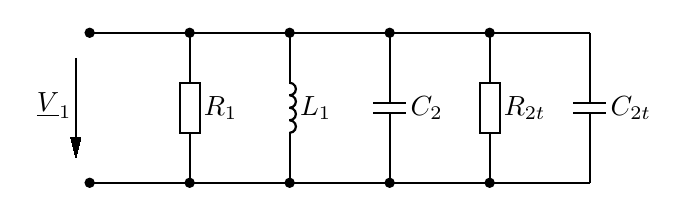
\begin{tikzpicture}[scale=2.54]%
% dpic version 2024.01.01 option -g for TikZ and PGF 1.01
\ifx\dpiclw\undefined\newdimen\dpiclw\fi
\global\def\dpicdraw{\draw[line width=\dpiclw]}
\global\def\dpicstop{;}
\dpiclw=0.8bp
\dpiclw=0.8bp
\dpicdraw[fill=black](0,0) circle (0.007874in)\dpicstop
\dpicdraw[fill=black](0,-0.75) circle (0.007874in)\dpicstop
\filldraw[line width=0bp](-0.094185,-0.525)
 --(-0.069185,-0.625)
 --(-0.044185,-0.525) --cycle\dpicstop
\dpicdraw (-0.069185,-0.125)
 --(-0.069185,-0.602094)\dpicstop
\draw (-0.069185,-0.363547) node[left=-2bp]{$ \underline{V}_1$};
\dpicdraw (0,0)
 --(0.5,0)\dpicstop
\dpicdraw[fill=black](0.5,0) circle (0.007874in)\dpicstop
\dpicdraw (0.5,0)
 --(0.5,-0.25)\dpicstop
\dpicdraw (0.5,-0.5)
 --(0.55,-0.5)
 --(0.55,-0.25)
 --(0.45,-0.25)
 --(0.45,-0.5)
 --(0.5,-0.5)\dpicstop
\dpicdraw (0.5,-0.5)
 --(0.5,-0.75)\dpicstop
\draw (0.55,-0.375) node[right=-2bp]{$ R_1$};
\dpicdraw[fill=black](0.5,-0.75) circle (0.007874in)\dpicstop
\dpicdraw (0.5,0)
 --(1,0)\dpicstop
\dpicdraw[fill=black](1,0) circle (0.007874in)\dpicstop
\dpicdraw (1,0)
 --(1,-0.25)\dpicstop
\dpicdraw (1,-0.25)
 --(0.994444,-0.25)\dpicstop
\dpicdraw (1,-0.25)
 ..controls (1.011165,-0.25) and (1.021481,-0.255956)
 ..(1.027063,-0.265625)
 ..controls (1.032646,-0.275294) and (1.032646,-0.287206)
 ..(1.027063,-0.296875)
 ..controls (1.021481,-0.306544) and (1.011165,-0.3125)
 ..(1,-0.3125)\dpicstop
\dpicdraw (1,-0.3125)
 --(0.994444,-0.3125)\dpicstop
\dpicdraw (1,-0.3125)
 ..controls (1.011165,-0.3125) and (1.021481,-0.318456)
 ..(1.027063,-0.328125)
 ..controls (1.032646,-0.337794) and (1.032646,-0.349706)
 ..(1.027063,-0.359375)
 ..controls (1.021481,-0.369044) and (1.011165,-0.375)
 ..(1,-0.375)\dpicstop
\dpicdraw (1,-0.375)
 --(0.994444,-0.375)\dpicstop
\dpicdraw (1,-0.375)
 ..controls (1.011165,-0.375) and (1.021481,-0.380956)
 ..(1.027063,-0.390625)
 ..controls (1.032646,-0.400294) and (1.032646,-0.412206)
 ..(1.027063,-0.421875)
 ..controls (1.021481,-0.431544) and (1.011165,-0.4375)
 ..(1,-0.4375)\dpicstop
\dpicdraw (1,-0.4375)
 --(0.994444,-0.4375)\dpicstop
\dpicdraw (1,-0.4375)
 ..controls (1.011165,-0.4375) and (1.021481,-0.443456)
 ..(1.027063,-0.453125)
 ..controls (1.032646,-0.462794) and (1.032646,-0.474706)
 ..(1.027063,-0.484375)
 ..controls (1.021481,-0.494044) and (1.011165,-0.5)
 ..(1,-0.5)\dpicstop
\dpicdraw (1,-0.5)
 --(0.994444,-0.5)\dpicstop
\dpicdraw (1,-0.5)
 --(1,-0.75)\dpicstop
\draw (1.03125,-0.375) node[right=-2bp]{$ L_1$};
\dpicdraw[fill=black](1,-0.75) circle (0.007874in)\dpicstop
\dpicdraw (1,0)
 --(1.5,0)\dpicstop
\dpicdraw[fill=black](1.5,0) circle (0.007874in)\dpicstop
\dpicdraw (1.5,0)
 --(1.5,-0.35)\dpicstop
\dpicdraw (1.416667,-0.35)
 --(1.583333,-0.35)\dpicstop
\dpicdraw (1.416667,-0.4)
 --(1.583333,-0.4)\dpicstop
\dpicdraw (1.5,-0.4)
 --(1.5,-0.75)\dpicstop
\draw (1.583333,-0.375) node[right=-2bp]{$ C_2$};
\dpicdraw[fill=black](1.5,-0.75) circle (0.007874in)\dpicstop
\dpicdraw (1.5,0)
 --(2,0)\dpicstop
\dpicdraw[fill=black](2,0) circle (0.007874in)\dpicstop
\dpicdraw (2,0)
 --(2,-0.25)\dpicstop
\dpicdraw (2,-0.5)
 --(2.05,-0.5)
 --(2.05,-0.25)
 --(1.95,-0.25)
 --(1.95,-0.5)
 --(2,-0.5)\dpicstop
\dpicdraw (2,-0.5)
 --(2,-0.75)\dpicstop
\draw (2.05,-0.375) node[right=-2bp]{$ R_{2t}$};
\dpicdraw[fill=black](2,-0.75) circle (0.007874in)\dpicstop
\dpicdraw (2,0)
 --(2.5,0)\dpicstop
\dpicdraw (2.5,0)
 --(2.5,-0.35)\dpicstop
\dpicdraw (2.416667,-0.35)
 --(2.583333,-0.35)\dpicstop
\dpicdraw (2.416667,-0.4)
 --(2.583333,-0.4)\dpicstop
\dpicdraw (2.5,-0.4)
 --(2.5,-0.75)\dpicstop
\draw (2.583333,-0.375) node[right=-2bp]{$ C_{2t}$};
\dpicdraw (2.5,-0.75)
 --(0,-0.75)\dpicstop
\end{tikzpicture}%
